\documentclass[12pt]{article}
\usepackage[margin=1in]{geometry}
\usepackage{amsmath}
\usepackage{graphicx}

\title{E155 Final Project Proposal: $\mu$Mudd Mark V Debugging and Lab 6 Revision}
\author{Christopher Ferrarin and Kaveh Pezeshki}
\date{31 October 2018}

\begin{document}
	\begin{LARGE}
	\noindent
		E155 
		Final 
		Project 
		Proposal: 
		$\mu$Mudd 
		Mark V \\
		Debugging 
		and 
		Lab 
		6 
		Revision
	\end{LARGE}

	\vspace{0.2cm}
	
	\begin{large}
	Christopher Ferrarin and Kaveh Pezeshki
	
	31 October 2018
	\end{large}


\section{Project Goal}
The $\mu$Mudd Mark V design, integrating an Altera Cyclone IV and Atmel SAM4S, is currently nonfunctional. There is a known bug in JTAG wiring to the MCU, but it it unknown whether this is the only existing bug. This project will involve identifying and correcting bugs in the $\mu$Mudd Mark V, and reworking Lab 6 to fit the new board.

\section{Project Deliverables}

The following tasks will be completed in this project:

\begin{enumerate}
	\item Identifying blocking bugs in the $\mu$Mudd which completely prevent MCU programming and operation
	\item Determining and implementing a solution to the above bugs. This solution may take several forms, as described below
	\item Reworking Lab 6 with instructor guidance to fit the new $\mu$Mudd MCU
\end{enumerate}

\subsection{Revised $\mu$Mudd}

We cannot yet explicitly state deliverables for the functional $\mu$Mudd PCB as they depend on unknown bugs in the design. Below are several potential deliverables, at least one of which will be provided at the end of the project:
\begin{enumerate}
	\item A modified version of the physical, pre-existing, $\mu$Mudd Mark V PCB that provides full MCU functionality
	\item Modified PCB design files that provide full MCU functionality
	\item A completed respin of the $\mu$Mudd with full MCU functionality
	\item A new JTAG cable that provides full MCU functionality
\end{enumerate}

\subsection{Reworked Lab 6 Requirements}

To maintain the IoT theme of the current lab 6, our reworked lab will include:

\begin{enumerate}
	\item Wireless connectivity (Bluetooth, WiFi, etc)
	\item Serial communication ($\text{I}^2\text{C}$, SPI, UART, etc) between the MCU and another device
	\item C programming for the MCU
	\item A practical use-case for the completed lab
\end{enumerate} 

\hspace{-0.8cm} While lab specifics will be determined after meeting with the instructor, we suggest the following:

\subsection{Reworked Lab 6 Proposal}

The reworked lab 6 will provide a wireless light sensor. Students will interface the $\mu$Mudd Mark V MCU with a photodiode and BlueSMiRF to relay temperature data over a bluetooth connection hosting a transparent serial link. This serial link will connect the MCU to a character or graphics LCD display through another BlueSMiRF. This introduces students to two new pieces of hardware: the BlueSMiRF and the serial display. A point of extra credit is available for adding more sensors, such as a thermistor, or for adding a novel feature to the project. The following block diagram illustrates the completed lab:

\begin{center}
	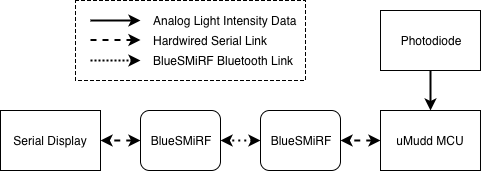
\includegraphics[width=10cm]{lab6_proposal}
\end{center}


\section{Project Budget}

The project budget is also ill-defined at this stage, as it depends on unknown bugs in the current design. I estimate the project will require a reference board for the SAM4S MCU, a respin of the current board, and an unknown set of new equipment and components, which may include a JTAG adapter and/or a replacement MCU. Also included are new components for the proposed lab 6. A preliminary budget is described below, with costs estimated from previous board development purchase orders or online vendors.

\begin{center}
	\begin{tabular}{llll}
	Item Name & Item Description & Vendor & Item Cost \\
	\hline
	SAM3-P256 & SAM3S Development Board & Olimex & \$31.09 \\
	ARM-USB-TINY-H & USB-JTAG Adapter & Olimex & \$47.86 \\
	PCB Fabrication &  & Advanced Circuits & \$264.00 \\
	ATSAM4S4BA-AU & SAM4S MCU & Digikey & \$3.93 \\
	2x BlueSMiRF Silver & Bluetooth Transceiver & Sparkfun & \$55.90 \\
	16x2 SerLCD & Serial Character LCD & Sparkfun & \$19.95 \\
	& & & \\
	Total Budget & & & \$422.19
	\end{tabular}

\end{center}


	
\end{document}